\documentclass[12pt,thmsa]{article}


%maths
\usepackage{amsmath}   % \sideset
\usepackage{amsthm}    % for proof
\usepackage{amsfonts}  % for \mathbb
\usepackage{mathrsfs}  % for Ralph Smith's Formal Script Font
\usepackage[mathscr]{euscript} %redefine the \mathcal command to use Euler script
\usepackage{amssymb}   % \varnothing, \bigstar, \blacksquare, \clubsuit, \blacktriangleright, \diamondsuit, \spadesuit, \dagger, \checkmark
\usepackage{optidef}   % for optimization definition

%algorithms
\usepackage{algorithm} % http://ctan.org/pkg/algorithms
\usepackage{algpseudocode}% http://ctan.org/pkg/algorithmicx

%tables
\usepackage{booktabs}  % Allows the use of \toprule, \midrule and \bottomrule in tables
\usepackage{multirow}
\usepackage{multicol}
\usepackage{tabularx}
\usepackage[table]{xcolor} % For \cellcolor
\usepackage[export]{adjustbox}

%figures
\usepackage{graphicx}  % Allows including images
\usepackage{float}     % Force figure placement in text with [H]

%tikzpicture
\usepackage{tikz}
\usepackage{scalerel}
\usepackage{pict2e}
\usepackage{tkz-euclide}
\usetikzlibrary{matrix}
\usetikzlibrary{shapes, positioning}
\usetikzlibrary{calc}
\usetikzlibrary{patterns, arrows.meta}
\usetikzlibrary{shadows}
\usetikzlibrary{external}

%pgfplots
\usepackage{pgfplots}
\pgfplotsset{compat=newest}
\usepgfplotslibrary{statistics}
\usepgfplotslibrary{fillbetween}

%colors
\usepackage{color}     % color

%other
\usepackage{cancel}
\usepackage{enumitem}
\setlist[itemize]{leftmargin=*} % global option, remove the indentation for a specific list
\usepackage{textcase}  % \MakeTextUppercase
\renewcommand{\qedsymbol}{$\blacksquare$} % change the QED symbol to a filled square
\usepackage{hyperref}

%layout
\usepackage{geometry}

\geometry{
	a4paper,
	total={170mm,257mm},
	left=20mm,
	right=20mm,
	top=20mm,
}

% Linhui added for newly defined color
\definecolor{forestgreen}{RGB}{34,139,34}

% Linhui added for Expectation and Variance
\newcommand{\Exp}{{\mathbb E}\! }
\newcommand{\Var}{\mbox{Var}\! }

% Linhui added for rename the command for empty set.
\let\oldemptyset\emptyset
\let\emptyset\varnothing

%------------------------------------------------------%
\makeatletter
\def\maketitle{%
	\par
	\hrule height 1.5pt\vspace{1ex}
	\par\noindent
	
	\begin{minipage}{0.5\textwidth}
		\scshape
		Purdue University \(\cdot\) ece 58000 \\[1ex]
		Optimization Methods \\
		Prof. Żak, Prof. Chong
	\end{minipage}
	\begin{minipage}{0.45\textwidth}
		\raggedleft
		\MakeTextUppercase{{\@title}}\\[0.3ex] % 0.2ex height space between two line
		\textit{\@author}\\[0.2ex]
		\textit{August 1, 2022}
	\end{minipage}
	\par\vspace{1ex}
	\hrule height 1.5pt\vspace{1ex}
	\par
}
\makeatother

\author{Linhui Xie}
\title{Lecture Note 01}
%------------------------------------------------------%

\begin{document}
\maketitle

\section{Mathematical preliminaries}

%------------------------------------------------------%
\subsection{Real vectors and matrices}

\subsubsection{Vectors}
\begin{itemize}
	\item \(\alpha, \beta, \gamma, ...\) : scalars.
	\item \(a_1, ..., a_n, x_1, ..., x_n, y_1, ..., y_n\) : real numbers, components of a vector, element of a set.
	\item \(\mathbb{R}\) : set of real numbers.
	
	\item \(\mathbb{R}^{n}\) : set of real column vectors.
	
\end{itemize}

\begin{equation*}
	\boldsymbol{x}=\left[\begin{array}{c}
		x_{1} \\
		\vdots \\
		x_{n}
	\end{array}\right], \quad x_{i} \in \mathbb{R}.
\end{equation*}

\begin{itemize}
	\item A \(n\)-dimensional \underline{column vector} and row vector,
\end{itemize}

\begin{equation*}
	\boldsymbol{a}=\left[\begin{array}{c}
		a_{1} \\
		a_{2} \\
		\vdots \\
		a_{n}
	\end{array}\right], \quad \boldsymbol{a}^{\top}=\left[a_{1}, a_{2}, \ldots, a_{n}\right].
\end{equation*}

\begin{itemize}
	\item Properties,
\end{itemize}

\begin{equation*}
	\begin{aligned}
		\boldsymbol{a}+\boldsymbol{b} & =\boldsymbol{b}+\boldsymbol{a}, & \alpha(\boldsymbol{a}+\boldsymbol{b}) & =\alpha \boldsymbol{a}+\alpha \boldsymbol{b}, \\
		(\boldsymbol{a}+\boldsymbol{b})+\boldsymbol{c} & =\boldsymbol{a}+(\boldsymbol{b}+\boldsymbol{c}), & \alpha(\beta \boldsymbol{a}) & =(\alpha \beta) \boldsymbol{a}, \\
		\mathbf{0} & =[0,0, \ldots, 0]^{\top}, & 1 \boldsymbol{a} & =\boldsymbol{a}, \\
		\boldsymbol{a}+\mathbf{0} & =\mathbf{0}+\boldsymbol{a}=\boldsymbol{a}, & \alpha \mathbf{0} & =\mathbf{0}=0 \boldsymbol{a}.
	\end{aligned}
\end{equation*}

\subsubsection{Matrices}

\begin{itemize}
	\item \(\mathbb{R}^{m \times n}:\) set of \(m \times n\) real matrices,
\end{itemize}

\begin{equation*}
	\boldsymbol{A}=\left[\begin{array}{cccc}
		a_{11} & a_{12} & \cdots & a_{1 n} \\
		a_{21} & a_{22} & \cdots & a_{2 n} \\
		\vdots & \vdots & \ddots & \vdots \\
		a_{m 1} & a_{m 2} & \cdots & a_{m n}
	\end{array}\right].
\end{equation*}

\begin{itemize}
	\item \(\mathbb{R}^{n \times 1}\) and \(\mathbb{R}^{n}\) as equivalent.
	
	\item \(\boldsymbol{A}^{\top}:\) transpose of \(\boldsymbol{A}\).
	
\end{itemize}

%------------------------------------------------------%
\subsection{Functions}
\begin{itemize}
	\item Set \(X: x \in X\).
	\item Function \(f: X \rightarrow Y\).
	
	\item \(f\) takes values in \(X\) and gives values in \(Y\).
	
	\begin{itemize}
	\item \(f(x)\) is the value of \(f\) at \(x\), where \(x \in X\).
	\end{itemize}

	\item A symbol \(:=\) denotes arithmetic assignment; \(x:=y\), means``\(x\) becomes \(y\)".
	
	\item A symbol \(\triangleq\) means ``equals by definition".
	
	\item Example: \(f: \mathbb{R}^{3} \rightarrow \mathbb{R}\),
	
\end{itemize}

\begin{equation*}
	f(\boldsymbol{x})=\frac{x_{1}^{2}+2 \log \left(x_{2} x_{3}\right) + x_{1}x_{2}x_{3}}{x_{2}}.
\end{equation*}


%------------------------------------------------------%
\subsection{Linear independence}
\begin{itemize}	
	\item A set of vectors \(\left\{\boldsymbol{a}_{1}, \ldots, \boldsymbol{a}_{k}\right\}\) is said to be \underline{linearly independent} if

	\begin{equation*}
		\alpha_{1} \boldsymbol{a}_{1}+\alpha_{2} \boldsymbol{a}_{2}+\cdots+\alpha_{k} \boldsymbol{a}_{k}=\mathbf{0},
	\end{equation*}
	
	implies that {\color{blue}all} the scalar coefficients \(\alpha_{i}, i=1, \ldots, k\), are equal to zero.
	
		\item A vector \(\boldsymbol{a}\) is said to be a \underline{linear combination} of vectors \(\boldsymbol{a}_{1}, \boldsymbol{a}_{2}, \ldots, \boldsymbol{a}_{k}\) if there are scalars \(\alpha_{1}, \ldots, \alpha_{k}\) such that
	
	\begin{equation*}
		\boldsymbol{a}=\alpha_{1} \boldsymbol{a}_{1}+\alpha_{2} \boldsymbol{a}_{2}+\cdots+\alpha_{k} \boldsymbol{a}_{k} .
	\end{equation*}

\end{itemize}

\begin{itemize}
	\item \(\mathcal{V}:\) a \underline{subspace} of \(\mathbb{R}^{n}\), if \(\mathcal{V}\) is closed for vector addition and scalar multiplication.
\end{itemize}


\begin{itemize}
	\item[\(\blacktriangleright\)] \(\mathscr{PROPOSITION}\) 2.1 A set of vectors \(\left\{\boldsymbol{a}_{1}, \boldsymbol{a}_{2}, \ldots, \boldsymbol{a}_{k}\right\}\) is \underline{linearly dependent} if and only if one of the vectors from the set is a linear combination of the remaining vectors.
\end{itemize}

\begin{itemize}
	\item The set of {\color{blue}all} linear combinations of \( \boldsymbol{a}_{1}, \boldsymbol{a}_{2}, \ldots, \boldsymbol{a}_{k} \) is called the \underline{span} of the vectors,
	\[ \operatorname{span}\left[\boldsymbol{a}_{1}, \boldsymbol{a}_{2}, \ldots, \boldsymbol{a}_{k}\right]=\left\{\sum_{i=1}^{k} \alpha_{i} \boldsymbol{a}_{i}: \alpha_{1}, \ldots, \alpha_{k} \in \mathbb{R}\right\}. \]
	
	\item Any set of linearly independent vectors \(\left\{\boldsymbol{a}_{1}, \boldsymbol{a}_{2}, \ldots, \boldsymbol{a}_{k}\right\} \subset \mathcal{V}\), is a \underline{basis} of the subspace \(\mathcal{V}\), if \(\mathcal{V}=\operatorname{span}\left[\boldsymbol{a}_{1}, \boldsymbol{a}_{2}, \ldots, \boldsymbol{a}_{k}\right]\).
	
	\item[\(\blacktriangleright\)] \(\mathscr{PROPOSITION}\) 2.2 If \(\left\{\boldsymbol{a}_{1}, \boldsymbol{a}_{2}, \ldots, \boldsymbol{a}_{k}\right\}\) is a basis of \(\mathcal{V}\), then any vector \(\boldsymbol{a}\) of \(\mathcal{V}\) can be represented uniquely as
	
	\begin{equation*}
		\boldsymbol{a}=\alpha_{1} \boldsymbol{a}_{1}+\alpha_{2} \boldsymbol{a}_{2}+\cdots+\alpha_{k} \boldsymbol{a}_{k},
	\end{equation*}
	
	where \(\alpha_{i} \in \mathbb{R}, i=1,2, \ldots, k\).
\end{itemize}

%------------------------------------------------------%
\subsection{Rank of a matrix}
\begin{itemize}
	\item The maximal number of linearly independent columns of \(\boldsymbol{A}\) is called the \underline{rank} of the matrix \(\boldsymbol{A}\), denoted rank \(\boldsymbol{A}\).
	
	\item[\(\blacktriangleright\)] \(\mathscr{PROPOSITION}\) 2.3 The rank of a matrix \(\boldsymbol{A}\) is \underline{invariant} under the following operations:
	
	\begin{itemize}
		\item \(\operatorname{rank}\left[\boldsymbol{a}_{1}, \ldots,  \alpha \boldsymbol{a}_{k}, \ldots, \boldsymbol{a}_{n}\right] = \operatorname{rank}\left[\boldsymbol{a}_{1}, \ldots,  \boldsymbol{a}_{k}, \ldots, \boldsymbol{a}_{n}\right],  \alpha \neq 0.\)
		
		\item \(\operatorname{rank}\left[\boldsymbol{a}_{1}, \ldots, \boldsymbol{a}_{k}, \ldots, \boldsymbol{a}_{l}, \ldots, \boldsymbol{a}_{n}\right] = \operatorname{rank}\left[\boldsymbol{a}_{1}, \ldots,  \boldsymbol{a}_{l}, \ldots, \boldsymbol{a}_{k}, \ldots, \boldsymbol{a}_{n}\right]. \)
		
		\item \(\operatorname{rank}\left[\boldsymbol{a}_{1}, \ldots, \boldsymbol{a}_{k} + (\alpha_{1}\boldsymbol{a}_{1} + \ldots + \alpha_{n}\boldsymbol{a}_{n}), \ldots, \boldsymbol{a}_{n}\right] = \operatorname{rank}\left[\boldsymbol{a}_{1}, \ldots,  \boldsymbol{a}_{k}, \ldots, \boldsymbol{a}_{n}\right].\)
	\end{itemize}
	
	\item The \underline{determinant} of the square matrix \(\mathbf{A}\), denoted \( \det \mathbf{A} \) or \( |\mathbf{A}| \). The determinant of a square matrix is a function of its columns,
	
	1. The determinant of the matrix \( \boldsymbol{A}=\left[\boldsymbol{a}_{1}, \boldsymbol{a}_{2}, \ldots, \boldsymbol{a}_{n}\right]\) is a linear function of each column; that is,
	\[
	\begin{array}{c}
		\operatorname{det}\left[\boldsymbol{a}_{1}, \ldots, \boldsymbol{a}_{k-1}, {\color{red}{\alpha}} \boldsymbol{a}_{k}^{(1)}+ {\color{blue}{\beta}} \boldsymbol{a}_{k}^{(2)}, \boldsymbol{a}_{k+1}, \ldots, \boldsymbol{a}_{n}\right] \\
		={\color{red}{\alpha}} \operatorname{det}\left[\boldsymbol{a}_{1}, \ldots, \boldsymbol{a}_{k-1}, \boldsymbol{a}_{k}^{(1)}, \boldsymbol{a}_{k+1}, \ldots, \boldsymbol{a}_{n}\right] 
		+{\color{blue}{\beta}} \operatorname{det}\left[\boldsymbol{a}_{1}, \ldots, \boldsymbol{a}_{k-1}, \boldsymbol{a}_{k}^{(2)}, \boldsymbol{a}_{k+1}, \ldots, \boldsymbol{a}_{n}\right],
	\end{array}
	\]
	for each \( \alpha, \beta \in \mathbb{R}, \boldsymbol{a}_{k}^{(1)}, \boldsymbol{a}_{k}^{(2)} \in \mathbb{R}^{n} \).
	
	2. If for some \(k\) we have \(\boldsymbol{a}_{k}=\boldsymbol{a}_{k+1}\), then
	\[\operatorname{det} \boldsymbol{A}=\operatorname{det}\left[\boldsymbol{a}_{1}, \ldots, \boldsymbol{a}_{k}, \boldsymbol{a}_{k+1}, \ldots, \boldsymbol{a}_{n}\right]=\operatorname{det}\left[\boldsymbol{a}_{1}, \ldots, \boldsymbol{a}_{k}, \boldsymbol{a}_{k}, \ldots, \boldsymbol{a}_{n}\right]=0\].
	
	3. Let
	\[
	\boldsymbol{I}_{n}=\left[\boldsymbol{e}_{1}, \boldsymbol{e}_{2}, \ldots, \boldsymbol{e}_{n}\right]=\left[\begin{array}{cccc}
		1 & 0 & \cdots & 0 \\
		0 & 1 & \cdots & 0 \\
		\vdots & \vdots & \ddots & \vdots \\
		0 & 0 & \cdots & 1
	\end{array}\right],
	\]
	where \( \left\{\boldsymbol{e}_{1}, \ldots, \boldsymbol{e}_{n}\right\} \) is the natural basis for \(\mathbb{R}^{n}\). Then
	\[
	\operatorname{det} \boldsymbol{I}_{n}=1.
	\]
	
	\item A \underline{\(p\)th-order minor} of an \({\color{red}{m}} \times {\color{blue}{n}}\) matrix \(\boldsymbol{A}\), with \(p \leq \min \{{\color{red}{m}}, {\color{blue}{n}}\}\), is the determinant of a \(p \times p\) matrix obtained from \(\boldsymbol{A}\) by deleting \(m-p\) rows and \(n-p\) columns.
	
	\item[\(\blacktriangleright\)] \(\mathscr{PROPOSITION}\) 2.4 If an \({\color{red}{m}} \times {\color{blue}{n}}\) matrix \(A({\color{red}{m}} \geq {\color{blue}{n}})\) has a nonzero \(n\)th-order minor, then the columns of \(A\) are linearly independent; that is, \(\operatorname{rank}(A)={\color{blue}{n}}\).
	
	\item The rank of a matrix is equal to the highest order of its nonzero \(\operatorname{minor}(\mathrm{s})\).
	
	\item A square matrix \(\boldsymbol{A} \in \mathbb{R}^{{\color{red}{n}} \times {\color{blue}{n}}}\) is \underline{nonsingular} or \underline{invertible} if rank \(\boldsymbol{A}={\color{blue}{n}}\) (full rank).
	
	\item A matrix is \underline{nonsingular} if and only if its determinant is nonzero.
	
\end{itemize}

%------------------------------------------------------%
\subsection{Linear equations}
\begin{itemize}
	\item[\(\spadesuit\)] \(\mathscr{THEOREM}\) 2.1 The system of equations \(\boldsymbol{A} \boldsymbol{x}=\boldsymbol{b}\) has a solution if and only if
	
	\begin{equation*}
		\operatorname{rank} \boldsymbol{A}=\operatorname{rank}[\boldsymbol{A}, \boldsymbol{b}] .
	\end{equation*}

	\item[\(\spadesuit\)] \(\mathscr{THEOREM}\) 2.2 Consider the equation \(\boldsymbol{A x}=\boldsymbol{b}\), where \(\boldsymbol{A} \in \mathbb{R}^{m \times n}\) and \(\operatorname{rank} \boldsymbol{A}=m\). A solution to \(\boldsymbol{A} \boldsymbol{x}=\boldsymbol{b}\) can be obtained by assigning arbitrary values for \(n-m\) variables and solving for the remaining ones.
\end{itemize}	

%------------------------------------------------------%
\subsection{Inner product and norm}
\subsubsection{Real domain}
\begin{itemize}
	\item Given \(\boldsymbol{x}, \boldsymbol{y} \in \mathbb{R}^{n}\).
	
	\item Define the \underline{Euclidean inner product} of \(\boldsymbol{x}\) and \(\boldsymbol{y}\) :
	
\end{itemize}

\begin{equation*}
	\langle\boldsymbol{x}, \boldsymbol{y}\rangle=\boldsymbol{x}^{\top} \boldsymbol{y}=\sum_{i=1}^{n} x_{i} y_{i}.
\end{equation*}

\begin{itemize}
	\item The inner product is a real-valued function \(\langle\cdot, \cdot\rangle: \mathbb{R}^{n} \times \mathbb{R}^{n} \rightarrow \mathbb{R}\),
	
	\begin{itemize}
		\item        \( \langle\boldsymbol{x}, \boldsymbol{x}\rangle \geq 0,\langle\boldsymbol{x}, \boldsymbol{x}\rangle=0 \) if and only if \(\boldsymbol{x}=\mathbf{0}\).
		
		\item      \(\langle\boldsymbol{x}, \boldsymbol{y}\rangle=\langle\boldsymbol{y}, \boldsymbol{x}\rangle\).
		
		\item        \(\langle\boldsymbol{x}+\boldsymbol{y}, \boldsymbol{z}\rangle=\langle\boldsymbol{x}, \boldsymbol{z}\rangle+\langle\boldsymbol{y}, \boldsymbol{z}\rangle\) .
		
		\item \(\langle r \boldsymbol{x}, \boldsymbol{y}\rangle=r\langle\boldsymbol{x}, \boldsymbol{y}\rangle\) for every \(r \in \mathbb{R}\).
	\end{itemize}
	Example,
	
	\begin{equation*}
		\langle\boldsymbol{A} \boldsymbol{x}, \boldsymbol{x}\rangle=
		\left( \boldsymbol{A} \boldsymbol{x} \right)^{\top} \boldsymbol{x} = 
		\boldsymbol{x}^{\top}  \boldsymbol{A}^{\top} \boldsymbol{x} = 
		\boldsymbol{x}^{\top}  \left(\boldsymbol{A}^{\top} \boldsymbol{x} \right) = 
		\left\langle\boldsymbol{x}, \boldsymbol{A}^{\top} \boldsymbol{x}\right\rangle.
	\end{equation*}
	
	
	\item Define the \underline{Euclidean norm} of \(\boldsymbol{x}\) :
	
\end{itemize}

\begin{equation*}
	\|\boldsymbol{x}\|=\sqrt{\langle\boldsymbol{x}, \boldsymbol{x}\rangle}=\sqrt{\boldsymbol{x}^{\top} \boldsymbol{x}}=\sqrt{\sum_{i=1}^{n} x_{i}^{2}}.
\end{equation*}


\begin{itemize}
	\item The Euclidean norm properties,
	\begin{itemize}
		\item \(\|\boldsymbol{x}\| \geq 0,\|\boldsymbol{x}\|=0\) if and only if \(\boldsymbol{x}=0\).
		
		\item \(\|\boldsymbol{x}\|=|r|\|\boldsymbol{x}\|, r \in \mathbb{R}\).
		
		\item \(\|\boldsymbol{x}+\boldsymbol{y}\| \leq\|\boldsymbol{x}\|+\|\boldsymbol{y}\|\).
	\end{itemize}
	\item[\(\spadesuit\)] \(\mathscr{THEOREM}\) 2.3 Cauchy-Schwarz Inequality. For any two vectors \(\boldsymbol{x}\) and \(\boldsymbol{y}\) in \(\mathbb{R}^{n}\), the Cauchy-Schwarz inequality holds,
	
	\begin{equation*}
		|\langle\boldsymbol{x}, \boldsymbol{y}\rangle| \leq\|\boldsymbol{x}\|\|\boldsymbol{y}\|.
	\end{equation*}	
	
\end{itemize}

\begin{itemize}
	
	\item The Euclidean norm is often referred to as the 2-norm, and denoted \(\|\boldsymbol{x}\|_{2} \). The norms above are special cases of the \(\boldsymbol{p}\)-\textbf{norm}, given by
	
	\[
	\|\boldsymbol{x}\|_{p}=\left\{\begin{array}{ll}
		\left(\left|x_{1}\right|^{p}+\cdots+\left|x_{n}\right|^{p}\right)^{1 / p} & \text { if } 1 \leq p<\infty \\
		\max \left\{\left|x_{1}\right|, \ldots,\left|x_{n}\right|\right\} & \text { if } p=\infty.
	\end{array}\right.
	\]
\end{itemize}
	
\begin{itemize}
	\item \(\boldsymbol{x}\) and \(\boldsymbol{y}\) are \underline{orthogonal} if \(\langle\boldsymbol{x}, \boldsymbol{y}\rangle=0\).
	
	\item A function \(f: \mathbb{R}^{n} \rightarrow \mathbb{R}^{m}\) is \underline{continuous} at \(x\) if for all \(\varepsilon>0\), there exists \(\delta>0\) such that \[\|\boldsymbol{y}-\boldsymbol{x}\|<\delta \Rightarrow\|\boldsymbol{f}(\boldsymbol{y})-\boldsymbol{f}(\boldsymbol{x})\|<\varepsilon.\]
	
\end{itemize}

\subsubsection{Complex domain}
\begin{itemize}
	\item An \underline{complex inner product} \(\langle\boldsymbol{x}, \boldsymbol{y}\rangle\) to be \(\sum_{i=1}^{n} x_{i} \bar{y}_{i}\) in complex vector space \(\mathbb{C}^{n}\), where the bar denotes complex conjugation. 
	
	\item The inner product on \(\mathbb{C}^{n}\) is a complex-valued function \(\langle\cdot, \cdot\rangle: \mathbb{C}^{n} \times \mathbb{C}^{n} \rightarrow \mathbb{C}\),
	
	\begin{itemize}
	\item \(\langle\boldsymbol{x}, \boldsymbol{x}\rangle \geq 0,\langle\boldsymbol{x}, \boldsymbol{x}\rangle=0\) if and only if \(\boldsymbol{x}=\mathbf{0}\). 
	
	\item \(\langle\boldsymbol{x}, \boldsymbol{y}\rangle=\overline{\langle\boldsymbol{y}, \boldsymbol{x}\rangle}\).
	
	\item \(\langle\boldsymbol{x}+\boldsymbol{y}, \boldsymbol{z}\rangle=\langle\boldsymbol{x}, \boldsymbol{z}\rangle+\langle\boldsymbol{y}, \boldsymbol{z}\rangle\).
	
	\item \(\langle r \boldsymbol{x}, \boldsymbol{y}\rangle=r\langle\boldsymbol{x}, \boldsymbol{y}\rangle\), where \(r \in \mathbb{C}\).
	\end{itemize}

	\item Deduction from above properties,
	\begin{equation*}
		\left\langle\boldsymbol{x}, r_{1} \boldsymbol{y}+r_{2} \boldsymbol{z}\right\rangle=\bar{r}_{1}\langle\boldsymbol{x}, \boldsymbol{y}\rangle+\bar{r}_{2}\langle\boldsymbol{x}, \boldsymbol{z}\rangle.
	\end{equation*}

	\item Define the \underline{Complex norm} of \(\boldsymbol{x}\) :

\end{itemize}

\begin{equation*}
\|\boldsymbol{x}\|=\sqrt{\langle\boldsymbol{x}, \boldsymbol{x}\rangle}=\sqrt{\boldsymbol{x}^{\top} \boldsymbol{x}}=\sqrt{\sum_{i=1}^{n} x_{i} \bar{x_{i}}}.
\end{equation*}



%------------------------------------------------------%
\subsection{Linear transformations}

\begin{itemize}
	\item A function \(\mathcal{L}: \mathbb{R}^{n} \rightarrow \mathbb{R}^{m}\) is called a \underline{linear transformation} if
	
	\begin{itemize}
		\item \(\mathcal{L}(a \boldsymbol{x})=a \mathcal{L}(\boldsymbol{x})\) for every \(\boldsymbol{x} \in \mathbb{R}^{n}\) and \(a \in \mathbb{R}\);
		\item \(\mathcal{L}(\boldsymbol{x}+\boldsymbol{y})=\mathcal{L}(\boldsymbol{x})+\mathcal{L}(\boldsymbol{y})\) for every \(\boldsymbol{x}, \boldsymbol{y} \in \mathbb{R}^{n}. \)
		
	\end{itemize}

	\item Let \(\left\{\boldsymbol{e}_{1}, \boldsymbol{e}_{2}, \ldots, \boldsymbol{e}_{n}\right\}\) and \(\left\{\boldsymbol{e}_{1}^{\prime}, \boldsymbol{e}_{2}^{\prime}, \ldots, \boldsymbol{e}_{n}^{\prime}\right\}\) be two bases for \(\mathbb{R}^{n}\). Define the \underline{transformation matrix} \(\boldsymbol{T}\) from \(\left\{\boldsymbol{e}_{1}, \boldsymbol{e}_{2}, \ldots, \boldsymbol{e}_{n}\right\}\) to  \(\left\{\boldsymbol{e}_{1}^{\prime}, \boldsymbol{e}_{2}^{\prime}, \ldots, \boldsymbol{e}_{n}^{\prime}\right\}\),
	
	\begin{equation*}
		\begin{gathered}
			{\left[ \begin{array}{cccc}
					% \vdots & \vdots &   & \vdots \\
					 &  &   &  \\
					\boldsymbol{e}_1 & \boldsymbol{e}_2 & \cdots & \boldsymbol{e}_n \\
					 &  &  & 
					% \vdots & \vdots &  & \vdots
				\end{array} \right] =
			\left[ \begin{array}{cccc}
				% \vdots & \vdots &   & \vdots \\
				 &  &   &  \\
				\boldsymbol{e}_1^{\prime} & \boldsymbol{e}_2^{\prime} & \cdots & \boldsymbol{e}_n^{\prime} \\
				 &  &   &
				% \vdots & \vdots &  & \vdots
			\end{array} \right] \boldsymbol{T}}.
		\end{gathered}
	\end{equation*}

	\item Given a vector \(\boldsymbol{v}\), \(\boldsymbol{x}\) is the coordinates of the vector with respect to a base \(\boldsymbol{B} =\left\{\boldsymbol{e}_{1}, \boldsymbol{e}_{2}, \ldots, \boldsymbol{e}_{n}\right\}\) and \(\boldsymbol{x}^{\prime}\) be the coordinates of the same vector with respect to a base \( \boldsymbol{B}^{\prime} = \left\{\boldsymbol{e}_{1}^{\prime}, \boldsymbol{e}_{2}^{\prime}, \ldots, \boldsymbol{e}_{n}^{\prime}\right\}\).
	\begin{equation*}
		\begin{gathered}
		\left[ \boldsymbol{v} \right]_{B}=x_1 \boldsymbol{e}_1+\cdots+x_n \boldsymbol{e}_n=\left[\boldsymbol{e}_1, \ldots, \boldsymbol{e}_n\right] \boldsymbol{x},  \\
		\left[ \boldsymbol{v} \right]_{B^{\prime}}=x_1^{\prime} \boldsymbol{e}_1^{\prime}+\cdots+x_n^{\prime} \boldsymbol{e}_n^{\prime} = \left[\boldsymbol{e}_1^{\prime}, \ldots, \boldsymbol{e}_n^{\prime}\right] \boldsymbol{x}^{\prime}, \\
		\boldsymbol{x}^{\prime} = \left[ \begin{array}{cccc}
			% \vdots & \vdots &   & \vdots \\
			 &  &   &  \\
			\boldsymbol{e}_1^{\prime} & \boldsymbol{e}_2^{\prime} & \cdots & \boldsymbol{e}_n^{\prime} \\
			 &  &   &  
			% \vdots & \vdots &  & \vdots
		\end{array} \right]^{-1}
		\left[ \begin{array}{cccc}
			% \vdots & \vdots &   & \vdots \\
			 &  &   &  \\
			\boldsymbol{e}_1 & \boldsymbol{e}_2 & \cdots & \boldsymbol{e}_n \\
			 &  &   &  
			% \vdots & \vdots &  & \vdots
		\end{array} \right] \boldsymbol{x}=\boldsymbol{T} \boldsymbol{x}.
		\end{gathered}
	\end{equation*}

	\item Example, let \(\boldsymbol{y}=\boldsymbol{A} \boldsymbol{x}\) and \(\boldsymbol{y}^{\prime}=\boldsymbol{A}^{\prime} \boldsymbol{x}^{\prime}\). Therefore,
	
	\begin{equation*}
		\boldsymbol{y}^{\prime}=\boldsymbol{T} \boldsymbol{y}=\boldsymbol{T} \boldsymbol{A} \boldsymbol{x}, 	\boldsymbol{y}^{\prime}=\boldsymbol{A}^{\prime} \boldsymbol{x}^{\prime}=\boldsymbol{A}^{\prime} \boldsymbol{T} \boldsymbol{x}.
	\end{equation*}
	
	and hence \(\boldsymbol{T} \boldsymbol{A}=\boldsymbol{A}^{\prime} \boldsymbol{T}\), or \(\boldsymbol{A}=\boldsymbol{T}^{-1} \boldsymbol{A}^{\prime} \boldsymbol{T}\).
	
	\item Two \(n \times n\) matrices \(\boldsymbol{A}\) and \(\boldsymbol{B}\) are \underline{similar} if there exists a nonsingular matrix \(\boldsymbol{T}\) such that \(\boldsymbol{A}=\boldsymbol{T}^{-1} \boldsymbol{B} \boldsymbol{T}\).

\end{itemize}


\begin{center}
	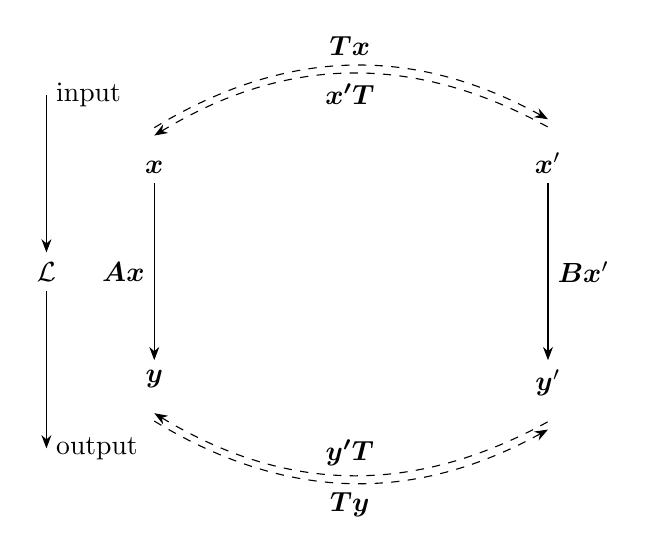
\begin{tikzpicture}[>=Stealth]
		% Nodes
		\node (L) {\(\mathcal{L}\)};
		\node [right=1cm of L] (pone) {};
		\node [above=1cm of pone] (x) {\(\boldsymbol{x}\)};
		\node [below=1cm of pone] (y) {\(\boldsymbol{y}\)};
		\node [right=6cm of L] (ptwo) {};
		\node [above=1cm of ptwo] (xprime) {\(\boldsymbol{x}'\)};
		\node [below=1cm of ptwo] (yprime) {\(\boldsymbol{y}'\)};
		
		% Input arrow
		\draw[->] ([yshift=2cm]L.north) -- (L.north) node[pos=0, right] {input};
		
		% Output arrow
		\draw[->] (L.south) -- ([yshift=-2cm]L.south) node[pos=1, right] {output};
		
		% Top dashed arrow
		\draw[->, dashed] ([yshift=3mm]x.north) to [bend left] node[above] {\(\boldsymbol{T}\boldsymbol{x}\)} ([yshift=3mm]xprime.north);
		\draw[<-, dashed] ([yshift=2mm]x.north) to [bend left] node[below] {\(\boldsymbol{x'}\boldsymbol{T}\)} ([yshift=2mm]xprime.north);
		
		% Bottom dashed arrow
		\draw[->, dashed] ([yshift=-3mm]y.south) to [bend right] node[below] {\(\boldsymbol{T}\boldsymbol{y}\)} ([yshift=-3mm]yprime.south);
		\draw[<-, dashed] ([yshift=-2mm]y.south) to [bend right] node[above] {\(\boldsymbol{y'}\boldsymbol{T}\)} ([yshift=-2mm]yprime.south);
		
		% top to botton arrow
		\draw[->] (x.south) -- (y.north) node[midway, left] {\(\boldsymbol{A}\boldsymbol{x}\)};
		\draw[->] (xprime.south) -- (yprime.north) node[midway, right] {\(\boldsymbol{B}\boldsymbol{x}'\)};
	\end{tikzpicture}
\end{center}

%------------------------------------------------------%
\subsection{Eigenvalues and eigenvectors}
\begin{itemize}
	\item Let \(\boldsymbol{A}\) be an \(n \times n\) square matrix.
	
	\item A scalar \(\lambda\) (possibly complex) and a nonzero vector \(\boldsymbol{v}\) satisfying the equation \(\boldsymbol{A} \boldsymbol{v}=\lambda \boldsymbol{v}\) are said to be, respectively, an eigenvalue and eigenvector of \(\boldsymbol{A}\).
	
	\item \(\lambda\) is an eigenvalue of \(\boldsymbol{A}\) if and only if \(\lambda \boldsymbol{I}-\boldsymbol{A}\) is singular (i.e., \(\operatorname{det}[\lambda \boldsymbol{I}-\boldsymbol{A}]=0\) ).
	
	\item \(\operatorname{det}[\lambda \boldsymbol{I}-\boldsymbol{A}]\) is called the \underline{characteristic polynomial} of \(\boldsymbol{A}\),
	
	\begin{equation*}
		\operatorname{det}[\lambda \boldsymbol{I}-\boldsymbol{A}]=\lambda^{n}+a_{n-1} \lambda^{n-1}+\cdots+a_{1} \lambda+a_{0}.
	\end{equation*}
	
	\item[\(\spadesuit\)] \(\mathscr{THEOREM}\) 3.1 Suppose that the characteristic equation \(\operatorname{det}[\lambda \boldsymbol{I}-\boldsymbol{A}]=0\) has \(n\) distinct roots \(\lambda_{1}, \lambda_{2}, \ldots, \lambda_{n}\). Then, there exist \(n\) linearly independent vectors \(\boldsymbol{v}_{1}, \boldsymbol{v}_{2}, \ldots, \boldsymbol{v}_{n}\) such that
	
	\begin{equation*}
		\boldsymbol{A} \boldsymbol{v}_{i}=\lambda_{i} \boldsymbol{v}_{i}, \quad i=1,2, \ldots, n.
	\end{equation*}

	\item[\(\spadesuit\)] \(\mathscr{THEOREM}\) 3.2 All eigenvalues of a real symmetric matrix are real.
	
	\item[\(\spadesuit\)] \(\mathscr{THEOREM}\) 3.3 If real \( n \times n\) matrix \(\boldsymbol{A}\) is symmetric, then a set of its eigenvectors forms an orthogonal basis for \(\mathbb{R}^{n}\).
	
	
\end{itemize}


%------------------------------------------------------%
\subsection{Orthogonal projections}
\begin{itemize}
	\item If \(\mathcal{V}\) is a subspace of \(\mathbb{R}^{n}\), then the \underline{orthogonal complement} of \(\mathcal{V}\), denoted by \(\mathcal{V}^{\perp}\), consists of all vectors that are orthogonal to every vector in \(\mathcal{V}\),
	\[\mathcal{V}^{\perp}=\left\{\boldsymbol{x}: \boldsymbol{v}^{\top} \boldsymbol{x}=0\right. \text{ for all }  \left.\boldsymbol{v} \in \mathcal{V}\right\}. \]
	
	\item \(\mathcal{V}\) and \(\mathcal{V}^{\perp}\) span \(\mathbb{R}^{n}\) in the sense that every vector \(\boldsymbol{x} \in \mathbb{R}^{n}\) can be represented uniquely as \(\boldsymbol{x}=\boldsymbol{x}_{1}+\boldsymbol{x}_{2}\), where \(\boldsymbol{x}_{1} \in \mathcal{V}\) and \(\boldsymbol{x}_{2} \in \mathcal{V}^{\perp}\).
	
	\item \(\boldsymbol{x}=\boldsymbol{x}_{1}+\boldsymbol{x}_{2}\) is the \underline{orthogonal decomposition} of \(\boldsymbol{x}\) with respect to \(\mathcal{V}\). \(\boldsymbol{x}_{1}\) and \(\boldsymbol{x}_{2}\) are \underline{orthogonal projections} of \(\boldsymbol{x}\) onto the subspaces \(\mathcal{V}\) and \(\mathcal{V}^{\perp}\), respectively.
	
	\item We write \(\mathbb{R}^{n}=\mathcal{V} \oplus \mathcal{V}^{\perp}\) and say that \(\mathbb{R}^{n}\) is a \underline{direct sum} of \(\mathcal{V}\) and \(\mathcal{V}^{\perp}\). 
	
	\item A linear transformation \(\boldsymbol{P}\) is an orthogonal projector onto \(\mathcal{V}\) if for all \(\boldsymbol{x} \in \mathbb{R}^{n}\) we have \(\boldsymbol{P} \boldsymbol{x} \in \mathcal{V}\) and \(\boldsymbol{x}-\boldsymbol{P} \boldsymbol{x} \in \mathcal{V}^{\perp}\).
\end{itemize}


\begin{itemize}
	\item Let \(\boldsymbol{A} \in \mathbb{R}^{m \times n}\), the \underline{range}, or image of \(\boldsymbol{A}\) is
	
	\begin{equation*}
		\mathcal{R}(\boldsymbol{A}) \triangleq\left\{\boldsymbol{A} \boldsymbol{x}: \boldsymbol{x} \in \mathbb{R}^{n}\right\}.  \quad \text { That's column space.}
	\end{equation*}
	
	The \underline{nullspace}, or \underline{kernel} of \(\boldsymbol{A}\) is
	
	\begin{equation*}
		\mathcal{N}(\boldsymbol{A}) \triangleq\left\{\boldsymbol{x} \in \mathbb{R}^{n}: \boldsymbol{A} \boldsymbol{x}=\mathbf{0}\right\}.
	\end{equation*}
	
	\(\mathcal{R}(\boldsymbol{A})\) and \(\mathcal{N}(\boldsymbol{A})\) are subspaces.
	
	\item[\(\spadesuit\)] \(\mathscr{THEOREM}\) 3.4 \(\mathcal{R}(\boldsymbol{A})^{\perp}=\mathcal{N}\left(\boldsymbol{A}^{\top}\right)\) and \(\mathcal{N}(\boldsymbol{A})^{\perp}=\mathcal{R}\left(\boldsymbol{A}^{\top}\right) \quad\) (That's row space. Together, four fundamental spaces in Linear Algebra.)
	
	\item If \(\boldsymbol{P}\) is an orthogonal projector onto \(\mathcal{V}\), then \(\boldsymbol{P} \boldsymbol{x}=\boldsymbol{x}\) for all \(\boldsymbol{x} \in \mathcal{V}\), and \(\mathcal{R}(\boldsymbol{P})=\mathcal{V}\).
	
	\item[\(\spadesuit\)] \(\mathscr{THEOREM}\) 03.05: A matrix \(\boldsymbol{P}\) is an orthogonal projector if and only if \(\boldsymbol{P}^{2}=\boldsymbol{P}=\boldsymbol{P}^{T}\).
\end{itemize}


%------------------------------------------------------%
\subsection{Symmetric matrices}
\begin{itemize}
	\item \(\boldsymbol{Q}\) is symmetric if \(\boldsymbol{Q}=\boldsymbol{Q}^{\top}\).
	
	\item A symmetric matrix \(\boldsymbol{Q}\) is said to be \underline{positive definite} if \(\boldsymbol{x}^{\top} \boldsymbol{Q} \boldsymbol{x}>0\) for {\color{red}all nonzero} vectors \(\boldsymbol{x}\).
	
	\item It is \underline{positive semi-definite} if \(\boldsymbol{x}^{\top} \boldsymbol{Q} \boldsymbol{x} \geq 0\) for {\color{red}all} \(\boldsymbol{x}\).
	
	\item Similarly, \underline{negative definite} and \underline{negative semi-definite},  if \(\boldsymbol{x}^{\top} \boldsymbol{Q} \boldsymbol{x}<0\) for {\color{red}all nonzero} vectors \(\boldsymbol{x}\), or \(\boldsymbol{x}^{\top} \boldsymbol{Q} \boldsymbol{x} \leq 0\) for {\color{red}all} \(\boldsymbol{x}\), respectively.
	
	\item For an \(n \times n\) symmetric real matrix \(\boldsymbol{Q}\),
	
	\begin{equation*}
		\begin{aligned}
			\boldsymbol{Q} \text{ positive-definite }  &  \Longleftrightarrow \quad \boldsymbol{x}^{\top} \boldsymbol{Q} \boldsymbol{x}>0 \text { for all } \boldsymbol{x} \in \mathbb{R}^n \backslash\{\boldsymbol{0}\} \\
			\boldsymbol{Q}  \text{ positive semi-definite } & \Longleftrightarrow \quad \boldsymbol{x}^{\top} \boldsymbol{Q} \boldsymbol{x} \geq 0 \text{ for all } \boldsymbol{x} \in \mathbb{R}^n \\
			\boldsymbol{Q} \text { negative-definite } & \Longleftrightarrow \quad \boldsymbol{x}^{\top} \boldsymbol{Q} \boldsymbol{x}<0 \text { for all } \boldsymbol{x} \in \mathbb{R}^n \backslash\{\boldsymbol{0}\} \\
			\boldsymbol{Q} \text { negative semi-definite } &\Longleftrightarrow \quad \boldsymbol{x}^{\top} \boldsymbol{Q} \boldsymbol{x} \leq 0 \text { for all } \boldsymbol{x} \in \mathbb{R}^n
		\end{aligned}
	\end{equation*}

	\item For an \(n \times n\) Hermitian complex matrix \(\boldsymbol{Q}\),
	\begin{equation*}
		\begin{aligned}
			\boldsymbol{Q} \text{ positive-definite }, \boldsymbol{Q} \succ 0 &  \Longleftrightarrow \quad
			\boldsymbol{x}^{\top} \boldsymbol{Q} \boldsymbol{x}>0 \text { for all } \boldsymbol{x} \in \mathbb{C}^n \backslash\{\boldsymbol{0}\} \\
			\boldsymbol{Q}  \text{ positive semi-definite }, \boldsymbol{Q}  \succeq 0 & \Longleftrightarrow \quad \boldsymbol{x}^{\top} \boldsymbol{Q} \boldsymbol{x} \geq 0 \text{ for all } \boldsymbol{x} \in \mathbb{C}^n \\
			\boldsymbol{Q} \text { negative-definite }, \boldsymbol{Q}  \prec 0 & \Longleftrightarrow \quad
			\boldsymbol{x}^{\top} \boldsymbol{Q} \boldsymbol{x}<0 \text { for all } \boldsymbol{x} \in \mathbb{C}^n \backslash\{\boldsymbol{0}\} \\
			\boldsymbol{Q} \text { negative semi-definite }, \boldsymbol{Q}  \preceq 0 &\Longleftrightarrow \quad \boldsymbol{x}^{\top} \boldsymbol{Q} \boldsymbol{x} \leq 0 \text { for all } \boldsymbol{x} \in \mathbb{C}^n
		\end{aligned}
	\end{equation*}
	
\end{itemize}


%------------------------------------------------------%
\subsection{Quadratic functions}
\begin{itemize}
	\item \(f: \mathbb{R}^{n} \rightarrow \mathbb{R}\) is a \underline{quadratic} function if

	\begin{equation*}
		f(\boldsymbol{x})=\boldsymbol{x}^{T} \boldsymbol{Q} \boldsymbol{x}+\boldsymbol{b}^{T} \boldsymbol{x}+c,
	\end{equation*}
	
	where \(\boldsymbol{Q}\) is {\color{red}symmetric}.
	
	\item If the matrix \(\boldsymbol{Q}\) is not symmetric, we can always replace it with the symmetric
	
	\begin{equation*}
		\begin{gathered}
			\boldsymbol{Q}_{0}=\boldsymbol{Q}_{0}^{T}=\frac{1}{2}\left(\boldsymbol{Q}+\boldsymbol{Q}^{T}\right) \\
			\boldsymbol{x}^{T} \boldsymbol{Q} \boldsymbol{x}=\boldsymbol{x}^{T} \boldsymbol{Q}_{0} \boldsymbol{x}=\boldsymbol{x}^{T}\left(\frac{1}{2} \boldsymbol{Q}+\frac{1}{2} \boldsymbol{Q}^{T}\right) \boldsymbol{x}
		\end{gathered}
	\end{equation*}
	
	\item The leading principal minors of matrix \(\boldsymbol{Q}\) are,

	\begin{equation*}
		\begin{gathered}
			\Delta_{1}=q_{11}, \quad \Delta_{2}=\operatorname{det}\left[\begin{array}{ll}
				q_{11} & q_{12} \\
				q_{21} & q_{22}
			\end{array}\right], 
			\Delta_{3}=\operatorname{det}\left[\begin{array}{lll}
				q_{11} & q_{12} & q_{13} \\
				q_{21} & q_{22} & q_{23} \\
				q_{31} & q_{32} & q_{33}
			\end{array}\right], \quad \ldots
		\end{gathered}
	\end{equation*}

	\item[\(\spadesuit\)] \(\mathscr{THEOREM}\) 3.6 Sylvester's Criterion. A quadratic form (\(\boldsymbol{Q}\) is symmetric) \(\boldsymbol{x}^{\top} \boldsymbol{Q} \boldsymbol{x}, \boldsymbol{Q}=\boldsymbol{Q}^{\top}\), is positive definite if and only if the leading principal minors of \(\boldsymbol{Q}\) are positive.
	
	\item A necessary condition for a real quadratic form to be positive semi-definite is that the leading principal minors be nonnegative. However, it is not a sufficient condition.
	
	\item A real quadratic form is positive semi-definite if and only if all principal minors are nonnegative.
	
	\item[\(\spadesuit\)] \(\mathscr{THEOREM}\) 3.7 A symmetric matrix \(\boldsymbol{Q}\) is positive definite (or positive semidefinite) if and only if all eigenvalues of \(\boldsymbol{Q}\) are positive (or nonnegative).

\end{itemize}

\begin{itemize}
	\item If \(\boldsymbol{Q}\) is positive definite, then \(f\) is a parabolic ``bowl".
\end{itemize}

\begin{center}
	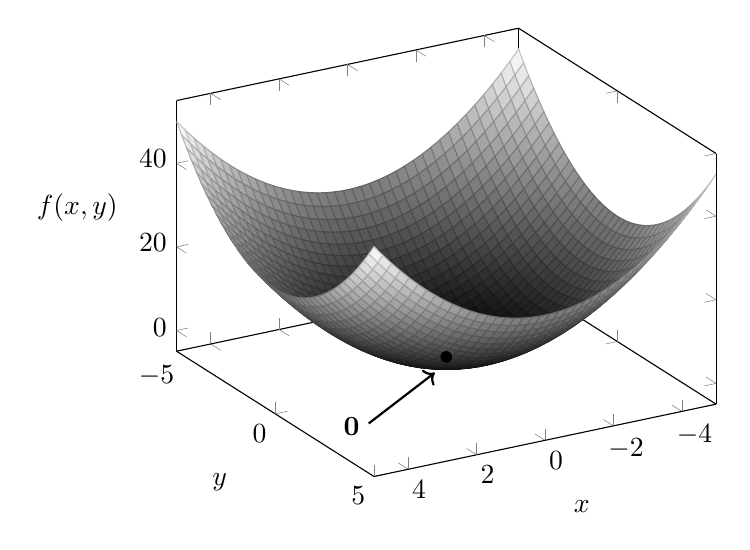
\begin{tikzpicture}
		\begin{axis}[
			xlabel = \(x\),
			ylabel = \(y\),
			zlabel = {\(f(x,y)\)},
			zlabel style={rotate=-90},
			% title = {Paraboloid: \(z = x^2 + y^2\) },
			view={150}{30}, % Set the viewing angle
			colormap/blackwhite,
			]
			
			% formula for parabolic bowl
			\addplot3[
			surf,
			domain=-5:5, % Set the domain for x
			domain y=-5:5, % Set the domain for y
			samples=40,
			] 
			{ x^2 + y^2 };
			
			% Point at the origin
			\node at (axis cs:0,0,0) [circle, fill, inner sep=1.5pt]{}; % Dot at origin
			\node at (axis cs:4.5, 3, 0) {\(\boldsymbol{0}\)};
			\draw [->, thick] (axis cs:4, 3, 0) -- (axis cs:0.8,0.8,0); % Arrow to origin
		\end{axis}
	\end{tikzpicture}
\end{center}

\begin{itemize}
	\item Quadratics simplify optimization, offering a clear structure for minimum or maximum solutions.
	
	\item Near optimal points, objective functions often resemble quadratics.
	
	\item Algorithms are more transparent when tested on quadratics.
	
	\item Insights from quadratic algorithm analysis extend to broader algorithmic applications.
	
\end{itemize}

%------------------------------------------------------%
\subsection{Matrix norm}

\begin{itemize}
	\item The \underline{norm of a matrix} \(\boldsymbol{A}\), denoted by \(\| \boldsymbol{A} \|\), satisfies
	
	\begin{itemize}
	\item[1.] \(\|\boldsymbol{A}\|>0\) if \(\boldsymbol{A} \neq \boldsymbol{O}\), and \(\|\boldsymbol{O}\|=0\), where \(\boldsymbol{O}\) is a matrix with all entries equal to zero.
	
	\item[2.]  \(\|c \boldsymbol{A}\|=|c|\|\boldsymbol{A}\|\), for any \(c \in \mathbb{R}\).
	
	\item[3.]  \(\|\boldsymbol{A}+\boldsymbol{B}\| \leq\|\boldsymbol{A}\|+\| \boldsymbol{B} \mid\).
	
	\end{itemize}

	\item For \(\boldsymbol{A} \in \mathbb{R}^{m \times n}\), an example of a matrix norm is the Frobenius norm, defined as
	
	\begin{equation*}
		\|\boldsymbol{A}\|_{F}=\left(\sum_{i=1}^{m} \sum_{j=1}^{n}\left(a_{i j}\right)^{2}\right)^{1 / 2}.
	\end{equation*}
	
	\item Note that the Frobenius norm is equivalent to the Euclidean norm on \(\mathbb{R}^{m \times n}\).
	
	\item For this course, only consider matrix norms satisfying the addition condition:
	
	\begin{itemize}
		\item[4.]\(\|\boldsymbol{A B}\| \leq\|\boldsymbol{A}\|\|\boldsymbol{B}\|\).
	\end{itemize}

	\item The Frobenius norm satisfies condition 4, \(\|\boldsymbol{A B}\|_{F} \leq\|\boldsymbol{A}\|_{F} \|\boldsymbol{B}\|_{F} \).
	
	\item Let \(\|\cdot\|_{(n)}\) and \(\|\cdot\|_{(m)}\) be vector norms on \(\mathbb{R}^{n}\) and \(\mathbb{R}^{m}\), respectively. The matrix norm is induced by, or is compatible with, the given vector norms if for any matrix \(\boldsymbol{A} \in \mathbb{R}^{m \times n}\) and any vector \(\boldsymbol{x} \in \mathbb{R}^{n}\), the following inequality is satisfied:
	
	\begin{equation*}
		\|\boldsymbol{A} \boldsymbol{x}\|_{(m)} \leq\|\boldsymbol{A}\|\|\boldsymbol{x}\|_{(n)}.
	\end{equation*}

	\item An induced matrix norm as
	
	\begin{equation*}
		\|\boldsymbol{A}\|=\max _{\|\boldsymbol{x}\|_{(n)}=1}\|\boldsymbol{A} \boldsymbol{x}\|_{(m)}.
	\end{equation*}

	\item For each matrix \(\boldsymbol{A}\) the maximum \(\max _{\|\boldsymbol{x}\|=1}\|\boldsymbol{A} \boldsymbol{x}\|\) is attainable; that is, a vector \(\boldsymbol{x}_{0}\) exists such that \(\left\|\boldsymbol{x}_{0}\right\|=1\) and \(\left\|\boldsymbol{A} \boldsymbol{x}_{0}\right\|=\|\boldsymbol{A}\|\).
	
	\item[\(\spadesuit\)] \(\mathscr{THEOREM}\) 3.8: Let
	
	\begin{equation*}
		\|\boldsymbol{x}\|=\left(\sum_{k=1}^{n}\left|x_{k}\right|^{2}\right)^{1 / 2}=\sqrt{\langle\boldsymbol{x}, \boldsymbol{x}\rangle}.
	\end{equation*}
	
	The matrix norm induced by this vector norm is
	
	\begin{equation*}
		\|\boldsymbol{A}\|=\sqrt{\lambda_{1}},
	\end{equation*}
	
	where \(\lambda_{1}\) is the largest eigenvalue of the matrix \(\boldsymbol{A}^{\top} \boldsymbol{A}\).
	
	\item Rayleigh's Inequality: If an \(n \times n\) matrix \(\boldsymbol{P}\) is real symmetric positive definite, then
	
	\begin{equation*}
		\lambda_{\min }(\boldsymbol{P})\|\boldsymbol{x}\|^{2} \leq \boldsymbol{x}^{T} \boldsymbol{P} \boldsymbol{x} \leq \lambda_{\max }(\boldsymbol{P})\|\boldsymbol{x}\|^{2},
	\end{equation*}
	
	where \(\lambda_{\min }(\boldsymbol{P})\) denotes the smallest eigenvalue of \(\boldsymbol{P}\), and \(\lambda_{\max }(\boldsymbol{P})\) denotes the largest eigenvalue of \(\boldsymbol{P}\). 
	
\end{itemize}

\medskip

\noindent
[Ref]: Edwin K.P. Chong, Stanislaw H. Żak, ``PART I MATHEMATICAL REVIEW" in ``\href{https://www.amazon.com/Introduction-Optimization-Edwin-K-Chong/dp/1118279018}{An introduction to optimization}", 4th Edition, John Wiley and Sons, Inc. 2013.


\end{document}
